\chapter{Resultados}
Nesse capítulo os resultados das diferentes soluções propostas no trabalho. Primeiramente introduzem-se as medidas de avaliação que serão utilizadas. Em seguida compara-se as etapas de classificação do método tradicional e híbrido, cujo processo de seleção de candidatos é idêntico, portanto a diferença em desempenho se dá apenas no classificador. Por fim avalia-se o desempenho do sistema completo das diferentes soluções apresentadas.

\section{Medidas de avaliação}
%https://sigarra.up.pt/feup/pt/pub_geral.show_file?pi_gdoc_id=365661 (termos recall e accuracy)
Para avaliar o desempenho das diferentes soluções apresentadas nesse trabalho se faz necessário a utilização de medidas que permitam comparar os resultados objetivamente e indicar facilmente os aspectos positivos e negativos relevantes de cada método. 

Em geral, num problema de classificação o indicador mais comum é a \textit{accuracy}, definida como a razão das classificações corretas pelo total de classificações. É fundamental notar, entretanto, que essa medida sozinha não é suficiente para avaliar um classificador, especialmente se o dataset for desbalanceado. Por exemplo, ao considerar um dataset com duas amostras negativas entre 20 e utilizar um classificador trivial que classifica qualquer amostra como sendo positiva, obtem-se uma precisão geral de 90\%, demonstrando que essa medida sozinha não é suficiente para avaliação.

Uma maneira compacta de representar a eficiência de um classificador é a \textbf{matriz de confusão}. Para uma classificação binária é uma matriz 2x2 em que a primeira linha indica as amostras falsas e a segunda as amostras verdadeiras. De forma semelhante, a primeira coluna indica amostras que foram classificadas como falsas e a segunda que foram classificadas como verdadeiras. Combinando-se essas linhas e colunas, obtém-se o número de verdadeiros negativos $TN$, falsos positivos $FP$, falsos negativos $FN$ e verdadeiros positivos $TP$, respectivamente.

\begin{table}[h]
\centering
\caption{Matriz de confusão}
\label{tab:matriz-confusão}
\begin{tabular}{ll|l|l|}
\cline{3-4}
                                            &   & \multicolumn{2}{l|}{Classificado} \\ \cline{3-4} 
                                            &   & 0               & 1               \\ \hline
\multicolumn{1}{|l|}{\multirow{2}{*}{Real}} & 0 & $TN$              & $FP$              \\ \cline{2-4} 
\multicolumn{1}{|l|}{}                      & 1 & $FN$              & $TP$              \\ \hline
\end{tabular}
\end{table}

Algumas grandezas utilizadas no campo de recuperação da informação \cite{inforetrival} são também úteis no contexto de classificação. O \textit{recall} é a fração de amostras positivas corretamente classificadas em relação ao número completo de amostras positivas do \textit{dataset}:
\begin{equation}
R = \frac{TP}{TP+FN}.
\end{equation}
A \textit{precision} fornece a fração das amostras positivas corretamente classificadas com relação à todas as amostras classificadas como positivas:
\begin{equation}
P = \frac{TP}{TP+FP}.
\end{equation}

Ambas as grandezas são importantes ao se avaliar um classificador, porém em uma aplicação específica uma delas pode ser mais relevante, como no caso desse trabalho. Para a indústria em questão é mais importante que a linha de produção se mantenha em funcionamento o maior tempo possível, portanto, deseja-se minimizar a quantidade de falsos positivos, que significam cabeças incorretamente identificadas que interrompem a produção sem necessidade. Nesse caso a medida de maior destaque será a \textit{precision}.

Outro aspecto a destacar na avaliação de classificadores é que não basta avaliar os indicadores apresentados apenas no \textit{dataset}. Isso acontece visto que o modelo pode ter se tornado muito específico para o conjunto de dados de treinamento, isto é, não generaliza bem, processo conhecido como \textit{overfitting}. Portanto, para medir o real desempenho do classificador utiliza-se de outro conjunto de dados supervisionados chamado de conjunto de validação -- \textit{validation set}, que não é utilizado para o treinamento do classificador.


\section{Classificadores}
\label{sec:resultados-classificadores}
O dataset foi gerado a partir de gravações realizadas no ambiente indústrial onde o sistema deverá ser instalado. A câmera foi posicionada num ponto próximo de onde deve ocorrer a sua instalação final. Diversos vídeos foram gravados e posteriormente analisados. Utilizando o algoritmo de detecção de candidatos visto em \ref{sec:tradicional-candidatos}, selecionou-se manualmente em cada quadro quais dos candidatos eram verdadeiramente cabeças. Repetindo esse processo em cada quadro formou-se um dataset, cuja amostra é o recorte do candidato, reduzido de 2459 amostras negativas (não cabeças) e 667 positivas (cabeças). Em seguida extendeu-se esse dataset reduzido para 9894 amostras negativas e 1222 positivas, formando o dataset completo. Criou-se, ainda, um conjunto de validação independente de 2738 amostras negativas e 235 amostras positivas.

\subsection{Método tradicional}
Avaliou-se o resultado das diferentes descritores mencionados em \ref{sec:tradicional-descritores} utilizando um processo de treinamento automático do SVM: varreu-se o espaço dos parâmetros $C$ entre $0.0001$ e $0.01$ com passos de $0.001$ e $\sigma$ entre $1$ e $100$ com passos de $5$. Os melhores resultados, selecionados segundo a medida de \textit{precision}, são apresentados na forma de matriz de confusão para cada um dos descritores.

\begin{table}[h]
\cfmat{Grades simples (7x7), dataset completo}{9881}{13}{36}{1186}
\cfmat{Grades simples (7x7), conjunto validação}{2445}{293}{181}{54}
\end{table}

Para o descritor de anéis concêntricos, primeiramente utilizou-se o dataset reduzido para avaliar qual a melhor dimensão do descritor, observando os seguintes resultados.

\begin{table}[h!]
\cfmat{Anéis concêntricos com 8 dimensões, dataset reduzido}{2364}{65}{185}{482}
\cfmat{Anéis concêntricos com 12 dimensões, dataset reduzido}{2344}{85}{183}{484}
\cfmat{Anéis concêntricos com 16 dimensões, dataset reduzido}{2385}{44}{111}{556}
\cfmat{Anéis concêntricos com 18 dimensões, dataset reduzido}{2410}{19}{60}{607}
\cfmat{Anéis concêntricos com 20 dimensões, dataset reduzido}{2359}{70}{141}{526}
\end{table}

Tendo visto que o melhor resultado foi obtido com 18 dimensões, utilizou-se o dataset completo para o treinamento e posterior avaliação através do conjunto de validação, como visto nas tabelas seguintes.

\begin{table}[h!]
\cfmat{Anéis concêntricos com 18 dimensões, dataset completo}{9859}{35}{213}{1009}
\cfmat{Anéis concêntricos com 18 dimensões, conjunto validação}{2573}{165}{116}{119}
\end{table}


\subsection{Classificador profundo}

\subsubsection{MLP}
Na estrutura MLP foram realizados testes com duas e três camadas intermediárias, com ativação RELU e um único perceptron de saída com ativação sigmoide indicando a probabilidade da amostra ser uma cabeça. Essa estrutura da saída como probabilidade é vantajosa pois permite ajustar o compromisso entre falso positivos e falso negativos do classificador, após treinamento, através da escolha do limiar de probabilidade $T$. Escolher um limiar mais alto significa exigir mais segurança do classificador e, portanto, reduzir o número de falsos positivos ao preço de possivelmente aumentar o número de falsos negativos.

Na configuração de duas camadas foram utilizados 512 e 256 perceptrons, respectivamente. Os resultados obtidos para o dataset e conjunto de validação foram os seguintes.
\begin{table}[h!]
\cfmat{MLP 2 camadas, $T=0.5$, dataset completo}{9805}{89}{100}{1122}
\cfmat{MLP 2 camadas, $T=0.9$, dataset completo}{9864}{30}{239}{983}

\cfmat{MLP 2 camadas, $T=0.5$, conjunto validação}{2644}{94}{45}{190}
\cfmat{MLP 2 camadas, $T=0.9$, conjunto validação}{2707}{29}{88}{147}
\end{table}

Para três camadas foram utilizados 1024, 512 e 256 perceptrons respectivamente, entretanto os resultados foram semelhantes aos obtidos com duas camadas, portanto o aumento em complexidade não é justificado visto que o desempenho permaneceu o mesmo.

\subsubsection{Redes convolucionais}
Para redes convolucionais utilizou-se uma única camada convolucional RELU com 16 núcleos 3x3 seguida por max-pooling (3x3) e uma camada densamente conectada de 128 percepetrons RELU e finalmente saída única com ativação sigmoide. Essa topologia foi a que teve o melhor desempenho, obtendo 100\% de \textit{accuracy} no conjunto de treinamento e 96.97\% no conjunto de validação, como observado a seguir.

\begin{table}[h!]
\cfmat{CNN, $T=0.5$, conjunto de validação}{2660}{78}{23}{212}
\cfmat{CNN, $T=0.9$, conjunto de validação}{2690}{48}{42}{193}
\end{table}

Tendo obtido o melhor desempenho até então, extendeu-se o conjunto de treinamento para 16898 amostras, das quais 14966 são negativas, e o processo de treinamento foi novamente efetuado, obtendo 99.9\% de \textit{accuracy} no treinamento e 97.54\% no conjunto de validação, como visto a seguir.

\begin{table}[h!]
\cfmat{CNN treinamento extendido, $T=0.5$, conjunto de validação}{2672}{66}{14}{221}
\cfmat{CNN treinamento extendido, $T=0.9$, conjunto de validação}{2686}{52}{21}{214}
\end{table}

Os resultados demonstram que essa topologia de rede é bastante eficiente para o problema em questão. Embora tenha ocorrido um aumento dos falsos positivos de 4 após extender o conjunto de treinamento, isso é justificável pela redução dos falsos negativos, que caiu pela metade, de 42 para 21.

\subsection{Discussão}
Para os diferentes classificadores observou-se as tabelas de confusão correspondentes. Porém essa comparação é facilitada através de um gráfico \textit{precision} x \textit{recall} como ilustra a figura \ref{fig:classifiers-results}. Deseja-se obter o melhor classificador, isto é, o classificador que maximize ambas as medidas de desempenho simultaneamente. 

Observa-se que muitos classificadores obtiveram um desempenho elevado no conjunto de treinamento, em especial as redes convolucionais que obtiveram \textit{accuracy} unitária, demonstrando a alta capacidade do modelo. Nota-se, entretanto, que há grande discrepância entre o desempenho dos classificadores no conjunto de treinamento e de validação, o que caracteriza \textit{overfitting}, e fica mais evidenciado nos métodos superficiais. Os métodos profundos, em contraste, apresentam uma boa generalização. Isso é explicado porque o modelo em questão foi corretamente especificado através no número de camadas e tamanho de filtros, de forma que sua capacidade se ajuste de forma adequada aos dados.

\begin{figure}[h]
\centering
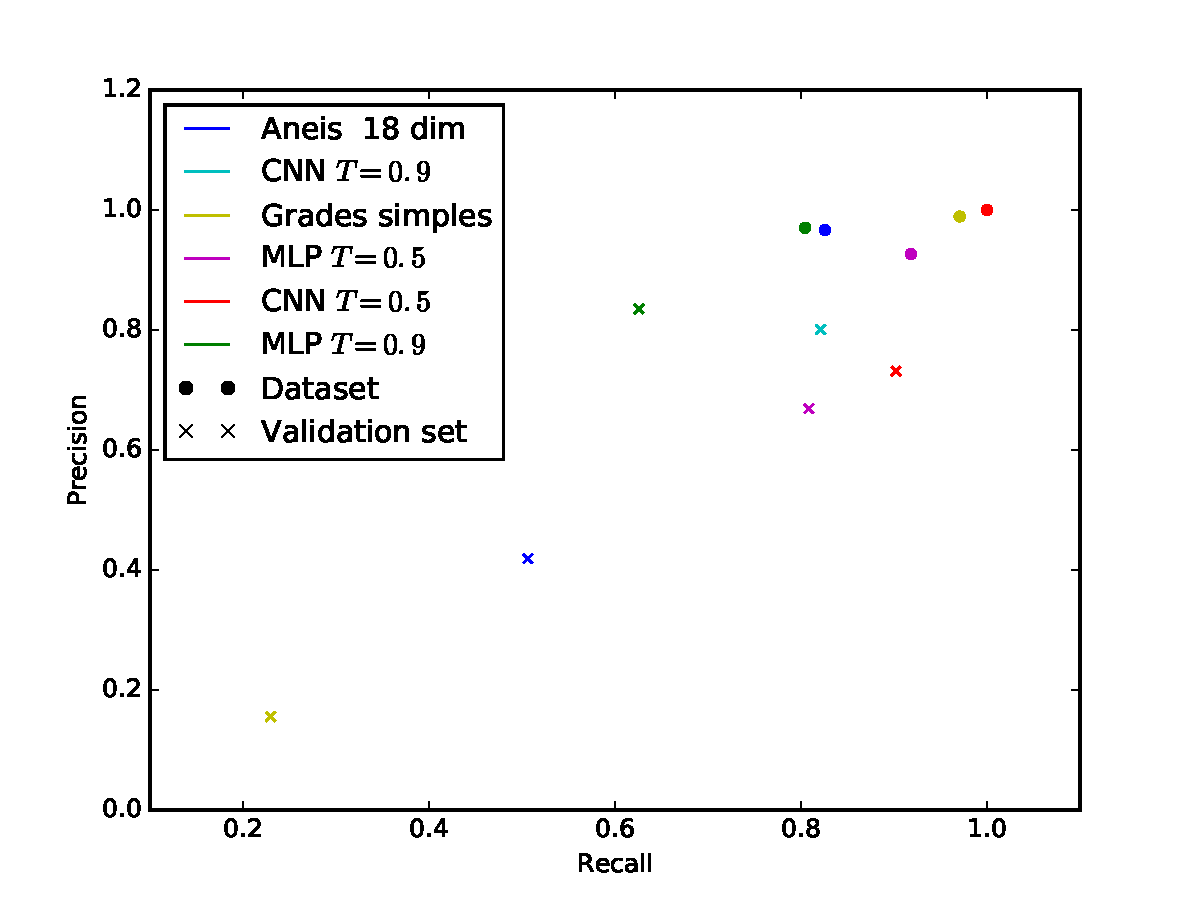
\includegraphics[width=0.8\textwidth]{results/prec_recall}
\caption{Gráfico comparativo de performance PxR dos classificadores}
\label{fig:classifiers-results}
\end{figure}

Outra forma de avaliar classificadores que oferecem uma saída probabilística é a curva ROC -- \textit{Receiver Operating Characteristic}, que no caso de classificadores demonstra como a taxa de verdadeiros positivos -- TVP (\textit{recall}) se relaciona com a taxa de falsos positivos -- TFP ($\frac{FP}{FP+TN}$) ao variar o limiar de probabilidade $T$ acima do qual se considera uma amostra como positiva. O melhor classificador indicaria uma taxa de TVP unitária com TFP nula, o que caracteriza uma reta de $(0,1)$ a $(1,1)$ delimitando área unitária. Portanto, quanto maior a área sob essa curva melhor o desempenho do classificador. Além disso, essa curva pode ser utilizada para selecionar o limiar de probabilidade $T$ de forma a atingir uma taxa de \textit{recall} especificada ao preço de uma TFP correspondente.

%https://en.wikipedia.org/wiki/Receiver_operating_characteristic

A figura \ref{fig:ROC} mostra um comparativo das curvas ROC dos classificadores MLP e CNN. Observa-se que as redes convolucionais garantem uma performance melhor visto ter maior área sob a curva, o que significa permitir uma TFP menor para uma mesma TVP.

\begin{figure}[ht]
\centering
\begin{subfigure}{.5\textwidth}
  \centering
  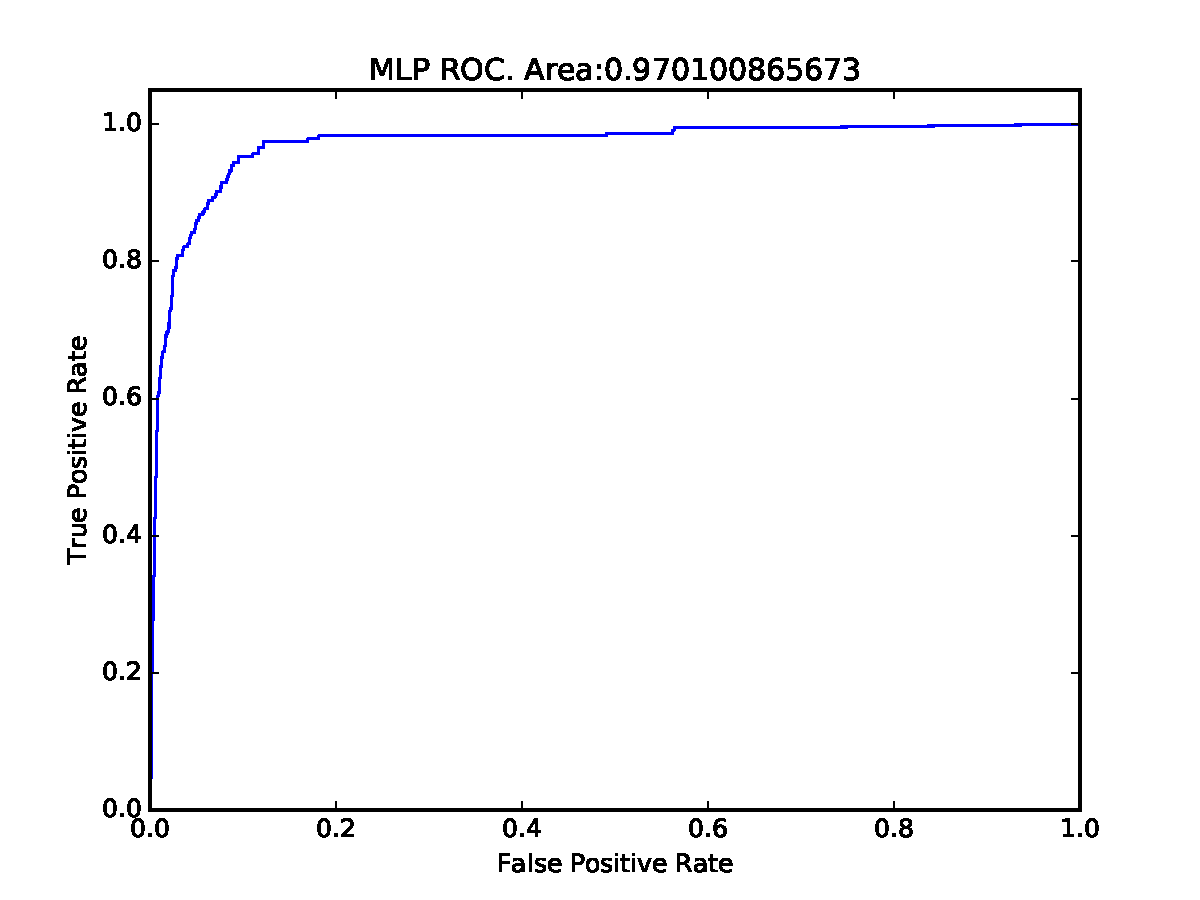
\includegraphics[width=\linewidth]{results/roc_mlp}
\end{subfigure}%
\begin{subfigure}{.5\textwidth}
  \centering
  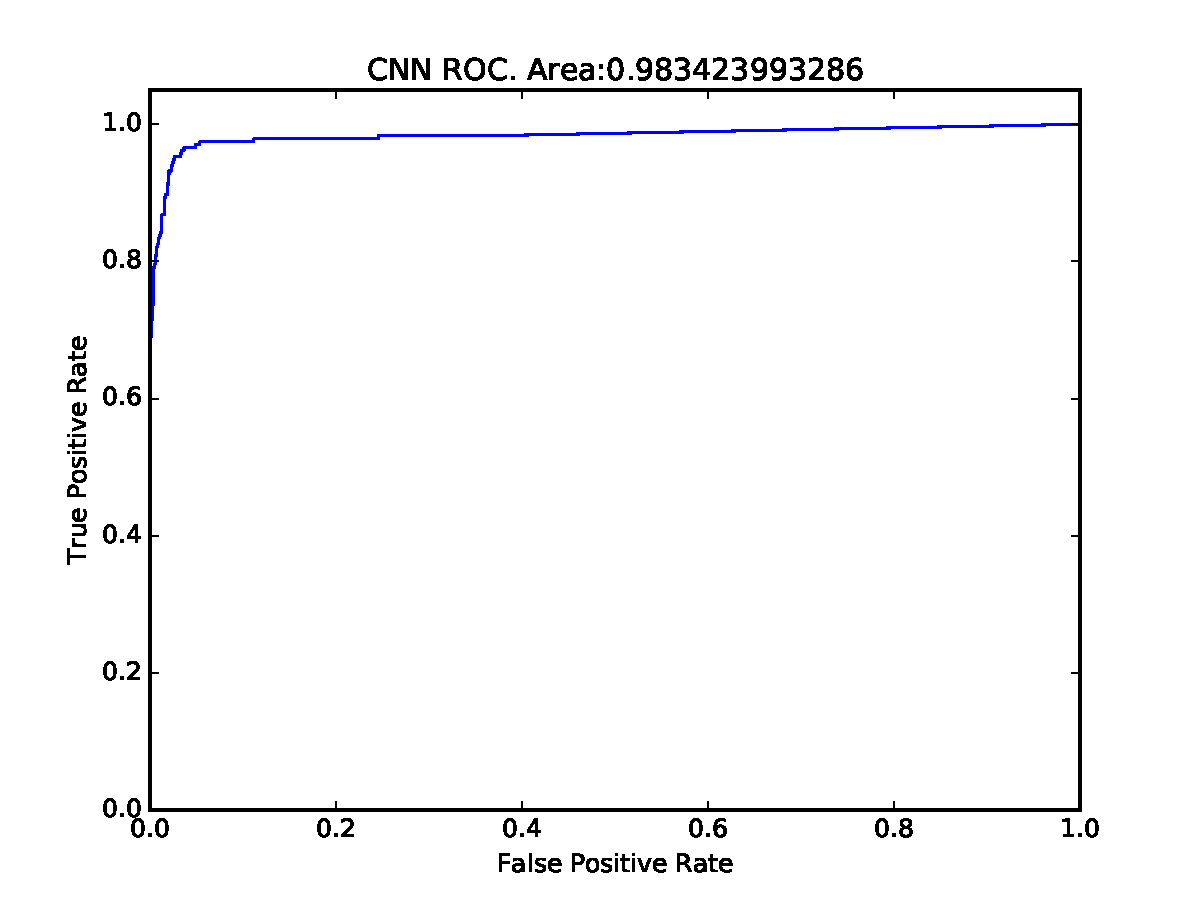
\includegraphics[width=\linewidth]{results/roc_cnn}
\end{subfigure}
\caption{Curva ROC dos classificadores MLP e CNN}
\label{fig:ROC}
\end{figure}

Conclui-se, então, que a melhor solução para classificação é a rede convolucional, oferencendo um bom compromisso entre \textit{recall} e \textit{precision} para a aplicação em questão, onde é mais importante que os falsos positivos sejam minimizados para evitar paralisação frequente da produção, portanto, é melhor ter uma \textit{precision} maior que \textit{recall}.

\section{Sistema completo}
Nessa seção serão comparados os resultados do sistema de extração de candidatos e de classificação como um todo. Tendo em vista os resultados da seção \ref{sec:resultados-classificadores}, a solução baseada na seleção de candidatos vista em \ref{sec:tradicional-candidatos} e classificador CNN apresentada no capítulo \ref{chap:class-profundo} será avaliada em detrimento das demais variações de classificadores. A última solução, cuja detecção e classificação são realizadas utilizando métodos profundos, vista no capítulo X também será avaliada.
